\documentclass{article}

\usepackage[margin = 1in]{geometry}

\usepackage{amsmath, graphicx}
\graphicspath{ {./images/} }

\title{Ch. 15 Solutions}
\author{Principles of Microeconomics}
\date{\today}

\begin{document}

\maketitle

\section*{Quick Quiz}

\begin{enumerate}

\item (c) -- Because there are many sellers all of whom offer the same product, firms are price takers in a perfectly competitive market.

\item (d) -- Marginal revenue is the price of the good. In a perfectly competitive industry, one firm increasing its quantity supplied doesn't change the price because all firms are price takers. Therefore, marginal revenue stays the same.

Total revenue equals price times quantity, so it's proportional to the quantity sold. If quantity increases by 10\%, total revenue increases by 10\%.

\item (b) -- If they chose a quantity for which $MC < MR$, they could increase their profit by producing one more unit because one more unit brings in more revenue than it costs them to produce. If they chose a quantity for which $MC > MR$, they could increase their profit by producing one less unit because their last unit brought in less revenue than it cost them to produce. Combined, that means they should produce the quantity at which $MC = MR$.

\item (d) -- The profit-maximizing quantity for a firm is the quantity at which marginal cost equals marginal revenue. In a competitive market, marginal revenue equals price, so the profit-maximizing quantity is the quantity at which price equals marginal cost. That means the marginal cost curve plots the profit-maximizing quantity for a firm at any given price. Since firms are profit-maximizers, that means the marginal cost curve plots the quantity supplied by a firm at any given price.

The caveat to that analysis is that a firm might be better off not producing at all. If a firm shuts down in the short run, it won't make any revenue, but it will save all of its variable costs. That means a firm is better off not producing in the short run if its revenue is less than its variable costs. With a little bit of math, we can show that that's the same thing as saying the firm is better off not producing in the short run if the market price is less than average variable cost:
	\begin{align*}
	TR &< VC \\
	\frac{TR}{Q} &< \frac{VC}{Q} \\
	\frac{PQ}{Q} &< AVC \\
	P &< AVC
	\end{align*}
Therefore, in the short run, if price is less than average variable cost, a firm will shut down, but if price is greater than average variable cost, a firm will produce the quantity given by the marginal cost curve. In other words, the firm's short-run supply curve is the marginal cost curve above its average variable cost curve.

\item (a) -- Firms produce the quantity at which marginal cost equals price, so if marginal cost is between average variable cost and average total cost, that means price is between average variable cost and average total cost.

If a firm shuts down in the short run, it will lose all of its revenue, but it will save all of its variable costs (it's fixed costs are sunk, so those are irrecoverable in the short run). Therefore, the firm will keep producing if its revenue is greater than its variable costs. That's the same thing as saying the firm will keep producing in the short run if price is greater than average variable cost. Since that's the case here, the firm continues to produce in the short run.

If a firm shuts down in the long run, it will lose all of its revenue, but it will save all of its costs (variable and fixed because the fixed costs become variable in the long run). Therefore, the firm will exit if its revenue is less than its costs. That's the same thing as saying the firm will exit in the long run if price is less than average total cost. Since that's the case here, the firm exits in the long run. 

\item (d) -- Firms will produce the quantity at which $P = MC$ because they're profit maximizers. They'll enter or exit the market until profits are zero which happens when $P = ATC$.

\item (c) -- Firms will produce the quantity at which $P = MC$ because they're profit maximizers. If new firms want to enter, profits must be positive which means $P > ATC$.

\item (c) -- In the short run, the tax is an increase in fixed costs. Since MC and AVC don't shift, it doesn't change firm's short run quantity produced, so the number of pretzels consumed stays the same. In the long run, firms exit the market because ATC shifts up which makes profit negative. When firms exit, the quantity produced decreases, so the number of pretzels consumed decreases.


\end{enumerate}

\section*{Questions for Review}

\begin{enumerate}

\item The two main characteristics are:
	\begin{itemize}
	
	\item the market has many buyers and sellers, and
	
	\item all of the sellers produce identical goods/services.
	
	\end{itemize}
	The third characteristic that economists only sometimes assume is:
	\begin{itemize}
	
	\item firms can freely enter and exit the market.
	
	\end{itemize}
	
\item A firm's revenue is the total amount of money that it brings in. A firm's profit is the total amount of money that it brings in minus its costs of production. Firms try to maximize profit. 

\item
	\begin{center}
	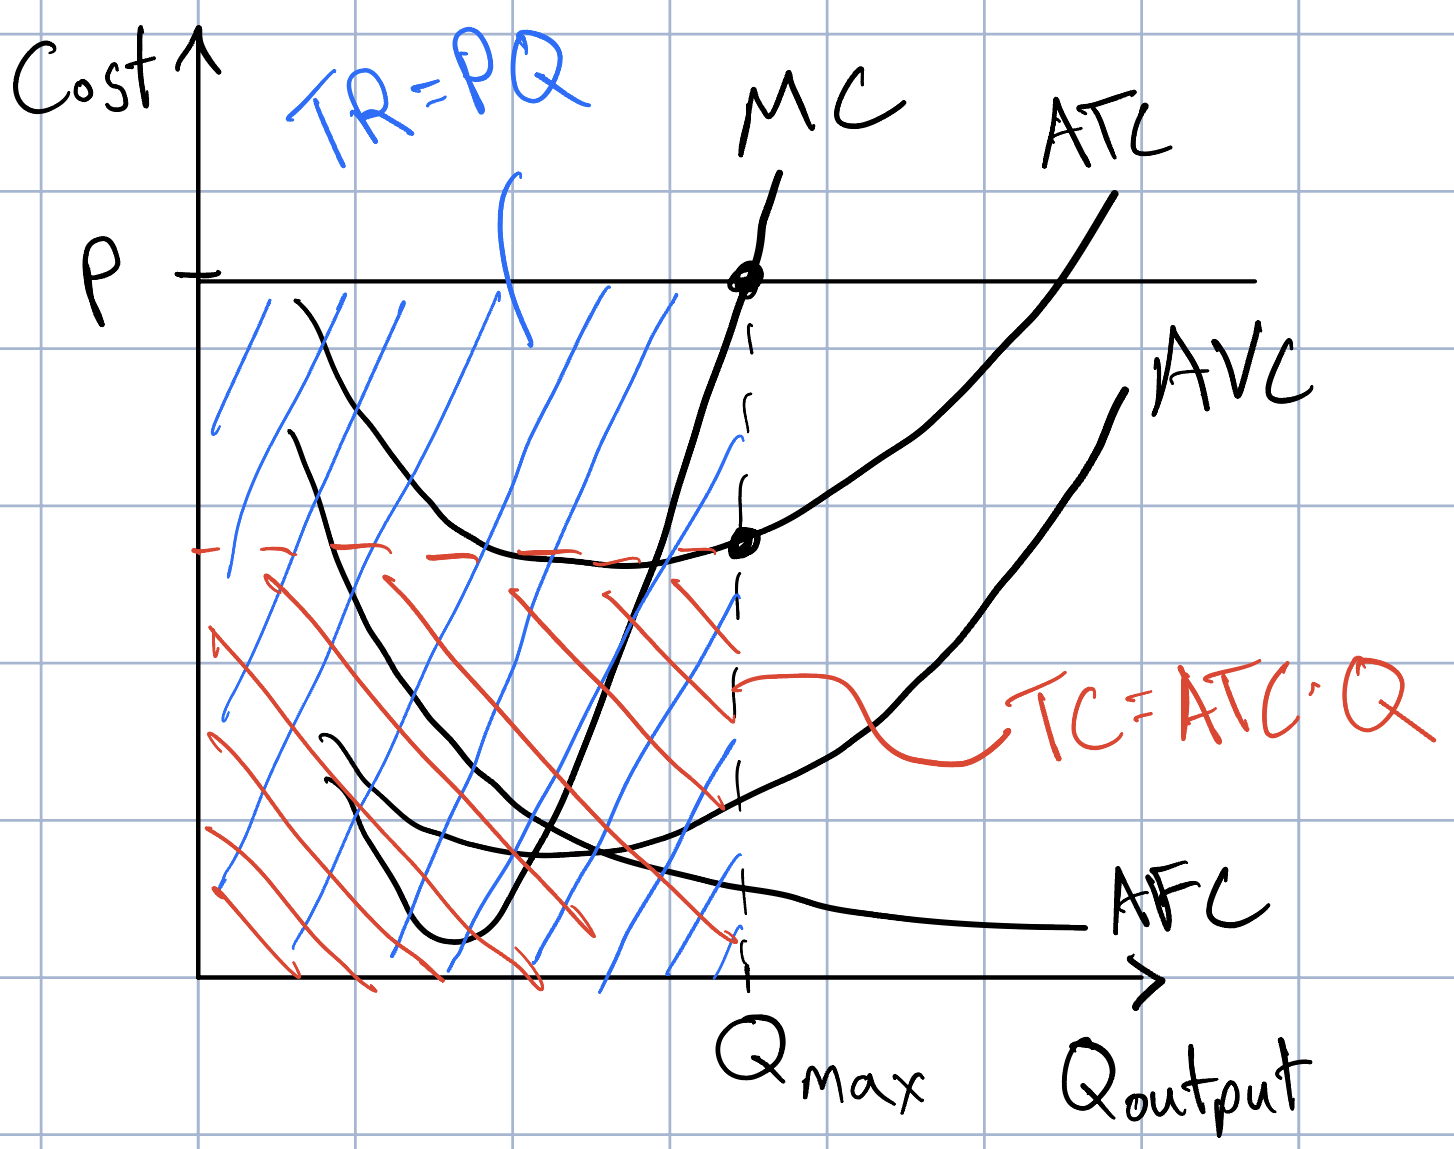
\includegraphics[width = 0.3\textwidth]{ch15_qfr3}
	\end{center}

\end{enumerate}

\section*{Problems and Applications}

\begin{enumerate}

\item 

	\begin{enumerate}
	
	\item An increase in the price of an input increases variable costs. As a result, marginal cost and average total cost shift up/left. The short run supply curve is the sum of all firms' marginal cost curves, so the short run supply curve shifts left as well. The long run supply curve is perfectly elastic at the price where firms make zero profit. Since that price increases when average total cost increases, the long run supply curve shifts up.
	
		\begin{center}
		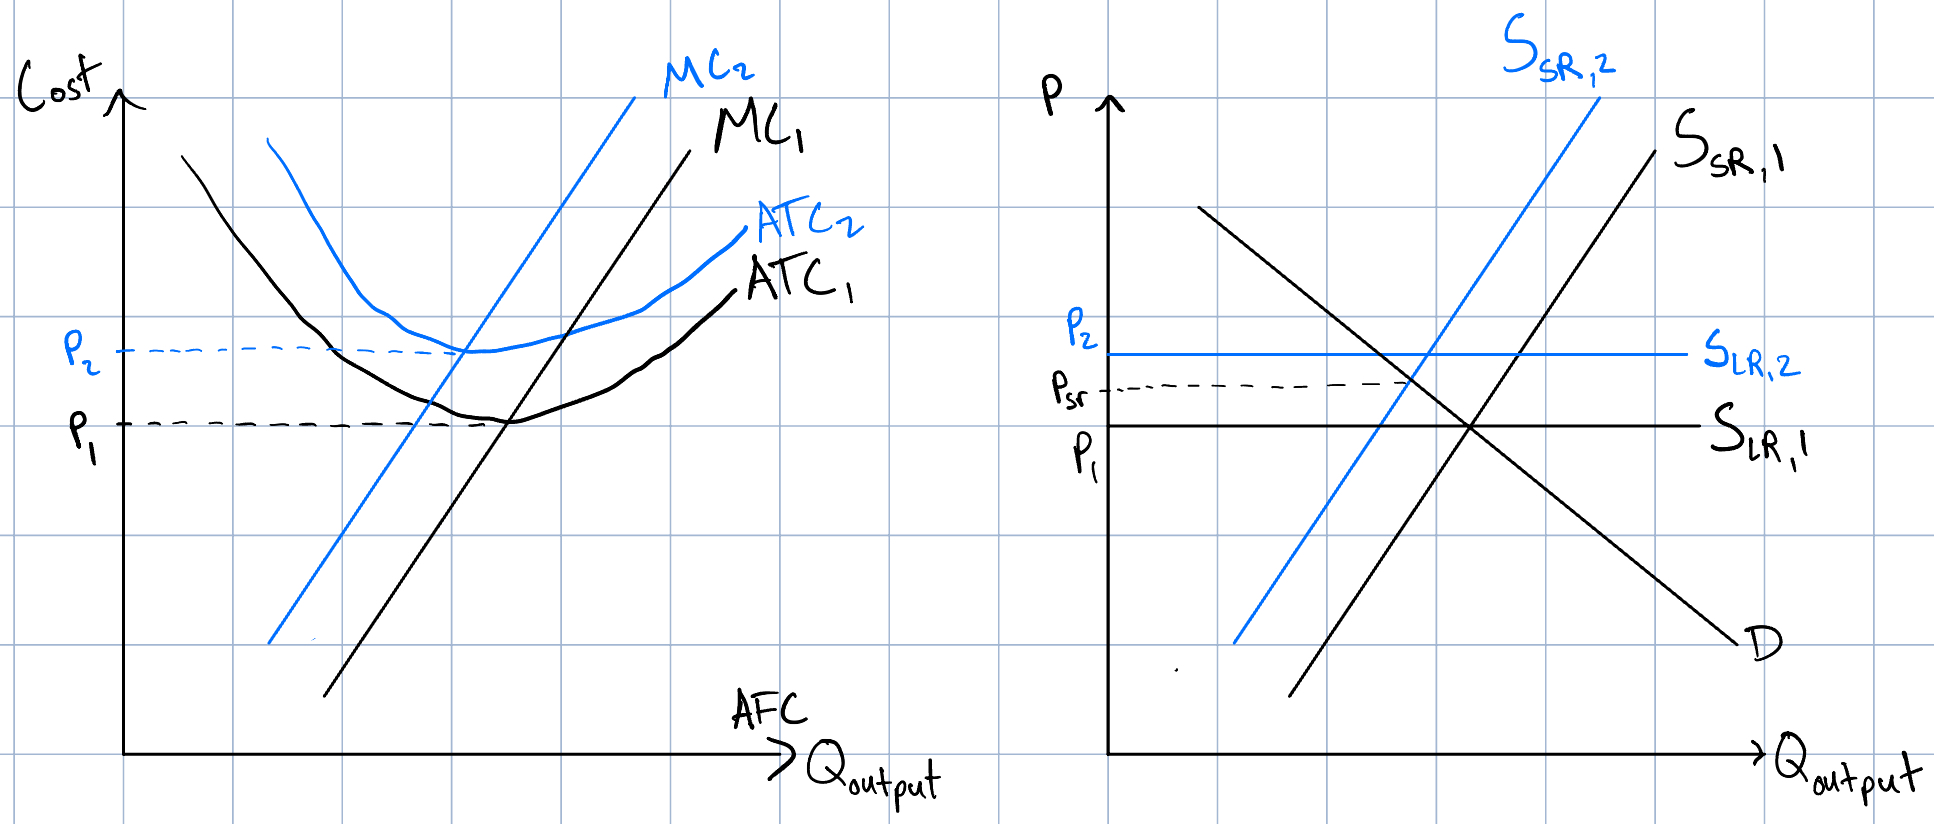
\includegraphics[width = 0.7\textwidth]{ch15_paa1a}
		\end{center}
		
	\item In the short run, profits depend on the elasticity of demand. As I drew it above, the short run price, $P_{SR}$, is below the new price at which firms make zero profit, $P_2$. In that case, profits become negative. If demand were more inelastic, $P_{SR}$ could be above the price at which firms make zero profit. In that case profits become positive. If profits become negative, the number of firms will decrease because some will exit the market. If profits become positive, the number of firms will increase because some will enter the market.
	
	\end{enumerate}
	
\item Leah's variable cost per day is \[\$280 - \$30 = \$250.\] Therefore, Leah's average variable cost is \[\$250 / 10 = \$25.\] That's less than her average revenue of \$27, so Leah produces in the short run.

	In the long run, Leah's average total cost is \[\$280 / 10 = \$28.\] That's greater than her average revenue, \$27, so Leah exits in the long run.
	
\item

	\begin{enumerate}
	
	\item The firm should produce 5 or 6 units.
	
		\begin{center}
		\begin{tabular}{c | c | c | c | c | c | c | c | c}
		\textbf{Quantity} & 0 & 1 & 2 & 3 & 4 & 5 & 6 & 7 \\
		\hline
		\textbf{Profit} & -8 & -1 & 6 & 13 & 19 & 21 & 21 & 19
		\end{tabular}
		\end{center}
		
	\item They intersect at a quantity of 5.5. That's consistent with my answer to (a). 
	
		\begin{center}
		\begin{tabular}{c | c | c | c | c | c | c | c | c}
		\textbf{Quantity} & 0 & 1 & 2 & 3 & 4 & 5 & 6 & 7 \\
		\hline
		\textbf{MR} & -- & 8 & 8 & 8 & 8 & 8 & 8 & 8 \\
		\hline
		\textbf{MC} & -- & 1 & 1 & 1 & 2 & 6 & 8 & 10
		\end{tabular}
		\end{center}
		
	\item It does look like the industry is competitive because marginal revenue is constant regardless of how much the firm produces. That implies that the firm is a price taker. The industry isn't in long run equilibrium because the firm has non-zero profit.
	
	\end{enumerate}
	
\item

	\begin{enumerate}
	
	\item \phantom{x}
	
		\begin{center}
		\begin{tabular}{| c | c | c | c | c | c | c | c |}
		\hline
		Q & FC & VC & AFC & AVC & ATC & MC & Profit \\
		\hline
		0 & 100 & 0 & -- & -- & -- & -- & -100 \\
		\hline
		1 & 100 & 50 & 100 & 50 & 150 & 50 & -100 \\
		\hline
		2 & 100 & 70 & 50 & 35 & 85 & 20 & -70\\
		\hline
		3 & 100 & 90 & 33.33 & 30 & 63.33 & 20 & -40 \\
		\hline
		4 & 100 & 140 & 25 & 35 & 60 & 50 & -40 \\
		\hline
		5 & 100 & 200 & 20 & 40 & 60 & 60 & -50\\
		\hline
		6 & 100 & 360 & 16.67 & 60 & 76.67 & 160 & -160\\
		\hline
		\end{tabular}
		\end{center}
		
	\item See the profit column above. No, shutting down is not a wise decision because their losses would be greater from shutting down than they would be from producing 4 cases.
	
	\item The firm's losses are \$100. It's not the best decision because if the firm produces 4 cases -- the other quantity at which marginal cost equals marginal revenue -- its losses are smaller, \$40. That's because the firm's marginal costs decline at first, so the firm's marginal costs are actually less than its marginal revenue for cases 2 \& 3. 
	
	\end{enumerate}
	
\item

	\begin{enumerate}
	
	\item I show the long run supply curve. In order to show the short run supply curve, you would have to add in the AVC curve.
	
		\begin{center}
		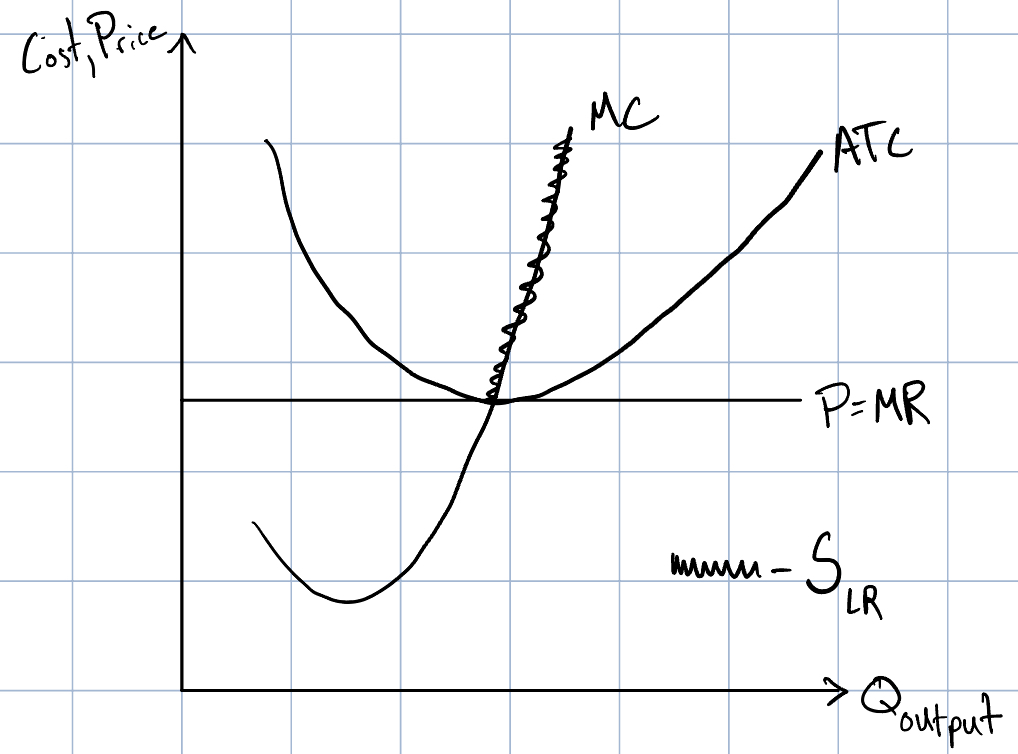
\includegraphics[width = 0.3\textwidth]{ch15_paa5a}
		\end{center}
		
	\item Hi-Tech's ATC curve shifts down, but all the other firms' ATC curves remain the same. Since it's a competitive market, Hi-Tech is a price taker, and the price of books remains the same. Profit is $(P - ATC)Q$, and $P - ATC$ increases, so Hi-Tech's profit increases.
	
	\item In the long run, when all the firms adopt the technology, all of their ATC curves shift down. Firms will enter or exit the market until price equals the minimum of the firms' ATC curves and profits equal zero. 
	
	\end{enumerate}
	
\item In a competitive market, all of a firm's output gets sold at the market price. That means marginal revenue is equal to average revenue which is equal to the market price of the good, Therefore, the average revenue and the price of the good both equal \$10. Since the price is \$10, that means the firm sold $\$500 / \$10 = \$50$

\item

	\begin{enumerate}
	
	\item Price equals average revenue which equals \$10. Therefore, profit is \[\pi = (P - ATC)*Q = (10 - 8)*100 = 200.\]
	
	\item Since the firm is profit maximizing, marginal cost equals marginal revenue which equals the price of the good, \$10.
	
	\item Average variable cost is 
	\[ AVC = ATC - AFC = ATC - FC/Q = 8 - 200/100 = \$6.\]
	
	\item Since marginal cost is greater than average total cost, average total cost is greater than its minimum. That means the firm's efficient scale is less than 100 units.
	
	\end{enumerate}
\item

	\begin{enumerate}
	
	\item Price is equal to marginal cost, greater than average variable cost, and less than average total cost. 
	
	\item \phantom{x}
	
		\begin{center}
		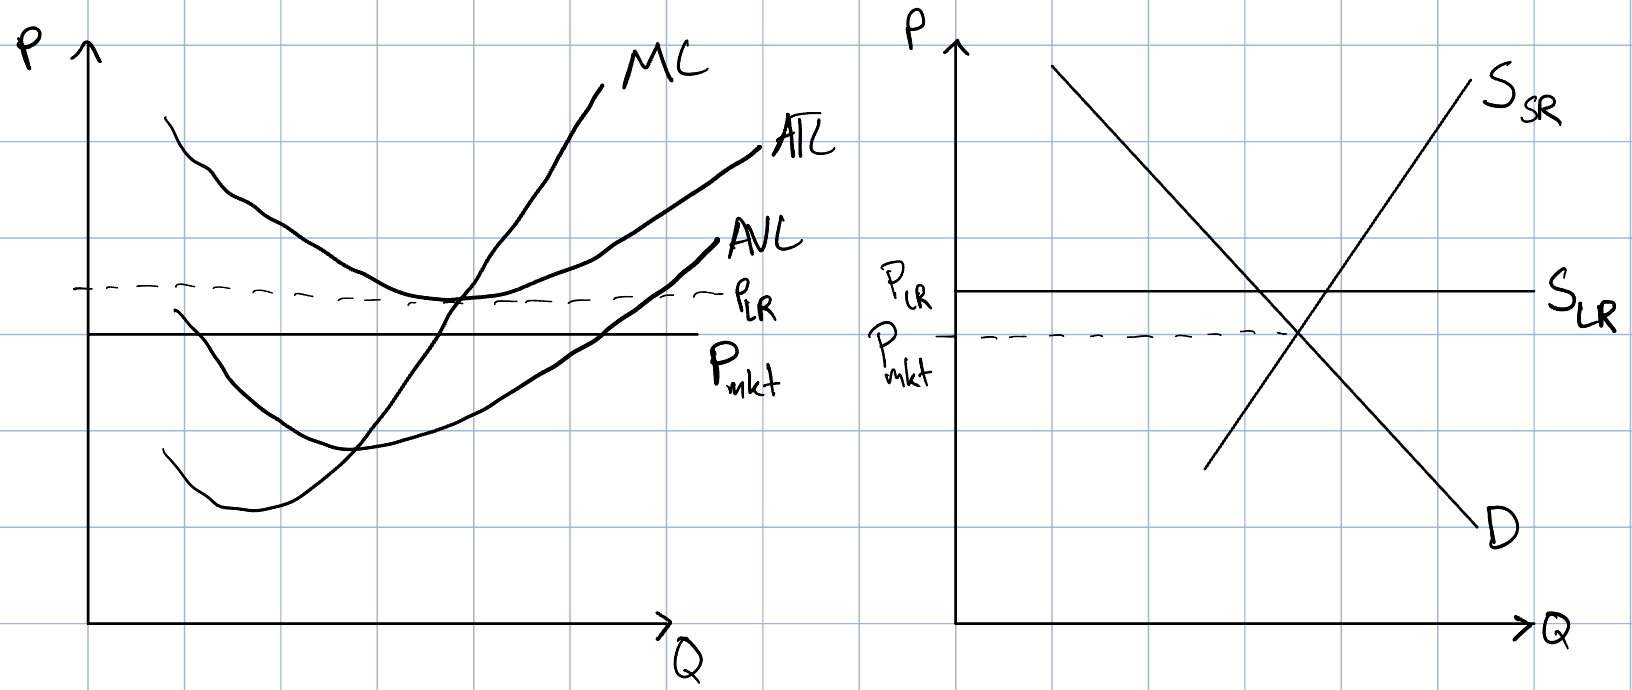
\includegraphics[width = 0.7\textwidth]{ch15_paa8b}
		\end{center}
		
	\item Firms leave the market because they are making losses. That decreases the number of suppliers which shifts short-run market supply left. When short-run market supply shifts left, price increases until profits are zero, and total quantity supplied decreases. The marginal cost and average total cost curves remain the same, so when price increases, firms start producing more. That means the quantity supplied by each firm still in the market increases.
	
	\end{enumerate}
	
\item 

	\begin{enumerate}
	
	\item \phantom{x}

		\begin{center}
		\begin{tabular}{c | c | c | c | c}
		Q & MC& VC & TC & ATC \\
		\hline
		1 pie & \$2 & \$2 & \$11 & \$11\\
		2 & 4 & 6 & 15 & 7.5 \\
		3 & 6 & 12 & 21 & 7 \\
		4 & 8 & 20 & 29 & 7.25 \\
		5 & 10 & 30 & 39 & 7.8 \\
		6 & 12 & 42 & 51 & 8.5
		\end{tabular}
		\end{center}
	
	\item When price is \$11, the market is in equilibrium at $Q = 200$. Each producer will make 5 pies because $P$ most closely equals $MC$ when $q = 5 \text{ or } 6$. When $q = 5$, profit is
	\begin{align*}
	Profit &= (P - ATC)Q \\
	&= (11 - 7.8)(5) \\
	&= 16.
	\end{align*}
	When $q = 6$, profit is
	\begin{align*}
	Profit &= (11 - 8.5)(6) \\
	&= 15.
	\end{align*}
	Since they earn more profit when $q = 5$, they'll produce 5. 
	
	\item No, it's not because there are non-zero profits.
	
	\item In the long run, they make zero profit. Price equals the minimum of average total cost which is approximately \$7 based on part (a). Price equals the minimum of average total cost when firms are producing 3 pies each. Based on the demand schedule, 600 pies are sold in the market which means that there are $600/3 = 200$ producers.
	
	\end{enumerate}
	
\item 

	\begin{enumerate}
	
	\item \phantom{x}
	
	\begin{center}
	\begin{tabular}{c | c | c | c | c}
	Q & AVC & VC & MC & ATC \\
	\hline
	1 & \$1 & \$1 & \$1 & \$17 \\
	2 & 2 & 4 & 3 & 10 \\
	3 & 3 & 9 & 5 & 8.33 \\
	4 & 4 & 16 & 7 & 8 \\
	5 & 5 & 25 & 9 & 8.2 \\
	6 & 6 & 36 & 11 & 8.67
	\end{tabular}
	\end{center}
	
	\item Each firm produces 5 units because $P$ most closely equals $MC$ when $q = 5 \text{ or } 6$. Profit is higher when $q = 5$ (\$9 vs. \$8), so the firm produces 5 units. The total quantity supplied is $Q_S = 100q = 500$.
	
	\item Because profits are positive, firms will enter the market. As the number of suppliers increases, supply will shift right.  A rightward shift in supply drives price down and quantity demanded up. The lower price leads to a lower quantity supplied by each firm because price will equal marginal cost at a point further left on the curve. 
	
	\item Based on part (a), the minimum average total cost is approximately \$8.
	
		\begin{center}
		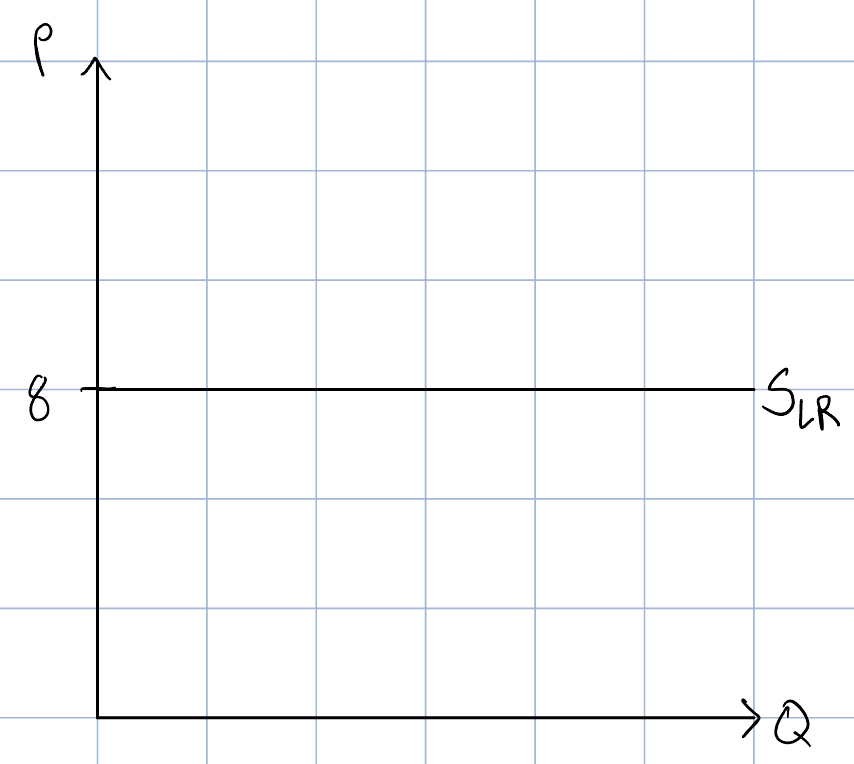
\includegraphics[width = 0.3\textwidth]{ch15_paa10c}
		\end{center}
	
	\end{enumerate}

\end{enumerate}

\section*{Non-Textbook Questions}

\begin{enumerate}

\item

\end{enumerate}

\end{document}